% ============================================================================================
% Section: Experimental Evaluation  (insert before the Conclusion; it becomes Section 8)
% Every number below is read from results/*.json through paper/evaluation_numbers.json;
% tables are generated by paper/make_tables.py. Figures: results/figures/*.pdf.
% ============================================================================================
\section{Experimental Evaluation}
\label{sec:eval}

% Plan: what is evaluated (H1-H4, RQ3, RQ4), from the consumer's view, and what was not executed.
This section tests hypotheses H1--H4 and questions RQ3 and RQ4 of the evaluation plan on the registries of
Table~1, from the consumer's side: toolkit size, context cost, coverage of the tools a task needs, reachable
unsafe services, and the cost of running and maintaining discovery. All results come from a
reference implementation of the capability model, Algorithms~1--3 and the certificate. No MCP server was
executed, so effects are judged against labelled ground truth rather than observed side effects
(Section~\ref{sec:eval-threats}).

\subsection{Experimental Setup}
\label{sec:eval-setup}

% Plan: data, splits and gold labels with exact counts.
\emph{Registries and tasks.} LiveMCPTool~\cite{mo2025livemcpbench} (69 servers, 525 tools) and
MCPToolBench++~\cite{fan2025mcptoolbench} (10 servers, 87 tools) are merged by \texttt{server::name} into 76
servers and 569 tools. The test split is the 95 LiveMCPBench tasks of the public release (Table~1 lists 94),
whose annotated tool chains give 256 gold tool mentions; 29 resolve to several \texttt{server::name}
identities, any of which counts, five name tools absent from the registry, and recall is computed over the 94
tasks with a resolvable gold tool. The MCPToolBench++ release holds 1,509 single-call requests (1,470 distinct
queries, against 1,429 in Table~1). Ten queries per category, 60 in total, form the development split on
which every parameter is tuned; all 1,509 requests are used where no analyst is involved.

% Plan: ground truth J, verifier, attacker; how J reaches the engine.
\emph{Ground truth, evidence and adversary.} The true effect relation $J$ was labelled once per tool by an
LLM (Claude Sonnet) from its name, description and schema, under a fixed guide that ignores annotations and
safety claims: scoped effects, whether the tool modifies persistent, shared or external state, and whether its
output can contain the principal's private data. Under $J$, 131 tools (23.0\%) modify state and 80 can return
private data. $J$ enters the engine only through a simulated sandbox verifier bound to $h(t)$, which reports
$J$'s effects and output labels truthfully except that it accepts a false read-only claim with a controlled
false-accept rate (FAR). Its records state a probe coverage $\kappa=0.9$ of the argument space, 30\% are
countersigned by a trusted attester, and it probes every tool except in the coverage sweep of
Section~\ref{sec:eval-h2}. As in Section~7, an attacker controls a fraction $\alpha$ of the servers, declares
all their tools read-only and non-destructive and launders their descriptions, but cannot alter verifier
evidence; it does not adapt to the policy.

% Plan: model profile and LLM roles.
\emph{Model profile and LLM roles.} $\rho_{\mathrm{LLM}}$ was measured for Claude Sonnet and Claude Haiku on
64 items: four classes (exact sum, exact count, majority sentiment, record look-up) $\times$
$n\in\{10,40,160,640\}$ $\times$ four items, answered from the data in context without tools, with an
isotonic fit and $\tau=0.9$. Sonnet answered all 64 correctly, including exact sums of 640 numbers; Haiku's
exact sum fell from 100\% at $n=40$ to 25\% at $n=160$ and 0\% at $n=640$. Rule~1 nevertheless fixes exact
classes below $\tau$ beyond $n=20$. Classes outside the calibration receive declared priors; treating them as
unknown (strict rule~2) is an ablation. The analyst role was run once with Sonnet on all 158 prompts (three
scenarios, 95 test, 60 development) and with Haiku on the 98 scenario and test prompts; the recorded goal
contracts are replayed, so every run is deterministic.

% Plan: implementation, parameters, three documented deviations.
\emph{Implementation and parameters.} Unless stated otherwise $K=5$, $d=2$,
$N_{\max}=40$, $u_{\min}=0.5$, $w_0=1$ and $\beta=\gamma=\delta=\eta=\zeta=0.5$ in Eq.~(6), $k_0=60$ in
Eq.~(5), and the trust policy assigns strengths $0.25$ (lex, raised to $0.45$--$0.50$ for delete, execute and
payment cues), $0.50$ (ann), $0.55+0.20\kappa$ (obs) and $1.0$ (att, trusted signer) against thresholds
$\ell_{\mathrm{lex}}=0.25$, $\ell_{\mathrm{ann}}=0.50$, $\ell_{\mathrm{obs}}=0.65$ and
$\ell_{\mathrm{att}}=0.90$. Three components deviate from Sections~6.1 and~6.3. The typing $\tau$ was
produced by the labelling pass from name, description and schema, not by structural typing with the
ontology, and was not checked against manually typed samples. The dense score uses a local latent-semantic
encoder (TF-IDF over word and character $n$-grams, 128 dimensions) because BGE-M3~\cite{chen2024bgem3} could
not be installed. Eq.~(6) gains a relevance term $w_{\mathrm{rel}}(1-\hat{s}(e))$, with $\hat{s}(e)$ the
candidate's fused retrieval score normalised per goal; $w_{\mathrm{rel}}=0$ recovers Eq.~(6), and
$w_{\mathrm{rel}}=10$ was selected on the development split. The flow bound (L) is checked conservatively:
every tool result enters the model's context and may reach any text-renderable argument of an egress tool.

% Plan: baselines, metrics, statistics (incl. multiplicity), experiment map.
\emph{Baselines, metrics and statistics.} Two approaches of Table~2 are re-implemented over the same registry
and retriever, RAG-MCP~\cite{gan2025ragmcp} (dense top-$k$ over the whole prompt) and
MCP-Zero~\cite{fei2025mcpzero} (server routing, then one tool per goal), beside per-subtask retrieval (one
tool per analyst goal) and the full catalogue; the baselines were not tuned. Metrics are toolkit size $|K|$,
tokens of the exposed tool definitions, gold-tool recall (the share of a task's gold tools in $K$), precision
over non-empty toolkits, abstention, exposure (the share of truly unsafe tools admitted), attack success and
latency. Means carry 95\% confidence intervals; paired comparisons over tasks use two-sided Wilcoxon
signed-rank tests with bootstrap intervals for the mean difference, and the ten such comparisons of
Section~\ref{sec:eval-h3} are Holm-adjusted ($p_{\mathrm{H}}$); proportions use Wilson intervals.
Table~\ref{tab:eval-design} lists the experiments and the kind of evidence each produces. Code, recorded LLM
outputs and raw results are available.\footnote{\url{https://github.com/msellamiTN/taas-provenance-discovery}}

\begin{table}[t]
\caption{Experiments and their evidence. Meas.: engine on registry data; LLM: recorded LLM role; Lab.:
LLM-labelled $J$; Sim.: simulated verifier or attacker; Syn.: generated registries.}
\label{tab:eval-design}
\centering\footnotesize\setlength{\tabcolsep}{3pt}
\begin{tabular}{@{}llp{3.5cm}l@{}}
\toprule
Exp. & Question & Conditions & Evidence\\
\midrule
E0 & H1 (registry) & 569 tools, annotations, $J$ & Meas., Lab.\\
E1 & H1 (behaviour) & sandbox traces & \emph{not run}\\
E2 & H2 & $\alpha\le0.5$, FAR $\le0.2$, 5 seeds & Meas., Lab., Sim.\\
E3 & H3 & 95 test, 60 dev.\ tasks & Meas., LLM\\
E4 & H4, Prop.~1 & 5 attack goals, 3 seeds & Meas., Lab., Sim.\\
E5 & RQ3 & 48 hidden typed chains & Syn.\\
E6 & Ablations & test split; 1,509 requests & Meas., LLM\\
E7 & RQ4 & $10^3$--$10^5$ tools, 600 events & Meas., Syn.\\
E8 & Typing, $\Theta$ & 525 tools, MCP-Bench input & Meas., LLM\\
\bottomrule
\end{tabular}
\end{table}

\subsection{Registry Characterisation (H1, Registry Level)}
\label{sec:eval-h1}

% Plan: Table 1 replicated, lexical evidence quality, H1 proper not tested.
The merged registry reproduces Table~1: 76 servers, 569 tools and 44 annotated tools, all from three servers
and all claiming \texttt{readOnlyHint=true}; under $J$ exactly one of them is not read-only. Requiring declared
read-only hints keeps 7.7\% of the registry, and reading a missing hint as safe removes nothing, because no tool
declares \texttt{readOnlyHint=false}. The share of state-modifying tools is 23.0\% under $J$ and 32.2\% under
the lexical labeller of Section~6.1 (precision 0.60, recall 0.84 against $J$, 21 unsafe tools missed),
bracketing the 27.8\% of Section~2.2; lexical evidence is thus both noisy and incomplete. H1 proper, a disagreement between declared and sandbox-observed
behaviour, requires executed servers and is not tested here.

\subsection{Provenance-Sound Eligibility (H2)}
\label{sec:eval-h2}

\begin{figure*}[t]
\centering
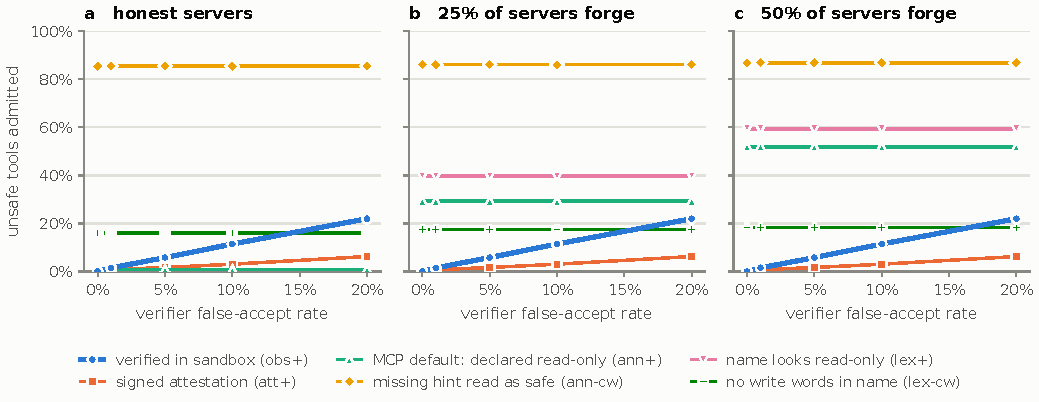
\includegraphics[width=\textwidth]{h2_exposure}
\caption{Exposure under a read-only policy: share of truly unsafe tools (under $J$) admitted by each
encoding, against the verifier's false-accept rate, when $\alpha=0$, $0.25$ and $0.5$ of the servers forge
metadata (569 tools, five seeds). Metadata-only encodings do not depend on the verifier.}
\label{fig:eval-h2}
\end{figure*}

% Plan: exposure numbers per encoding; Prop. 2 and Obs. 1 confirmed (by construction for obs+ at FAR 0).
Fig.~\ref{fig:eval-h2} compares six encodings of a read-only policy. MCP's default reading (ann$+$, admit
declared read-only tools) admits 0.8\% of the unsafe tools when every server is honest, 29.3\% when a quarter
forge their hints and 51.9\% when half do. Reading a missing hint as safe (ann-cw) admits 85.5\% even with
honest servers, as Observation~1 predicts for a registry in which almost no tool is annotated, and the lexical
encodings admit between 16.0\% and 59.4\%. Verified evidence (obs$+$) admits no unsafe tool at FAR 0 for every
$\alpha$, as Proposition~2(a) states (with a truthful simulated verifier this checks the implementation); its
exposure is independent of $\alpha$ and grows with the verifier's error, to 1.5\%, 5.8\%, 11.5\% and 22.0\% at
FAR of 1\%, 5\%, 10\% and 20\%.

% Plan: utility vs coverage; verifier-quality condition of Section 7 quantified; scope of the verdict.
Soundness costs utility through coverage, not forgery: at $\alpha=0.25$ and FAR 5\%, obs$+$ keeps every safe
tool when the verifier probes the whole registry (ann$+$ keeps 34.6\%), but only 24.4\% when it probes a
quarter of the tools, with exposure falling to 0.6\%. Section~7 asks for a false-accept rate well below the
error rate of the evidence replaced. With honest servers the declared hints here are almost all truthful, and a verifier at FAR 1\% (1.5\%)
is already worse than ann$+$ (0.8\%); once a quarter of the servers forge metadata, obs$+$ admits fewer unsafe
tools than ann$+$ at every tested FAR up to 20\%. H2 is supported for a non-adaptive metadata attacker and a
verifier whose only error is false acceptance.

\subsection{Model-Conditioned Gap Analysis (H3)}
\label{sec:eval-h3}

\begin{table}[t]
\caption{Toolkit size, context cost and gold-tool recall (H3): means over tasks, recall with 95\% CI. LMB:
LiveMCPBench test split (95 tasks; recall over the 94 with a resolvable gold tool). TB++: MCPToolBench++
development split (60 queries). Tok.: tokens of the raw definitions (name, description, schema) for every
system; TaaS's sanitised manifest needs 126 and 88 tokens.}
\label{tab:eval-h3}
\centering\footnotesize\setlength{\tabcolsep}{2.2pt}
\begin{tabular}{@{}lrrlrrl@{}}
\toprule
 & \multicolumn{3}{c}{LMB (test)} & \multicolumn{3}{c}{TB++ (dev)}\\
\cmidrule(lr){2-4}\cmidrule(l){5-7}
System & $|K|$ & Tok. & Recall & $|K|$ & Tok. & Recall\\
\midrule
TaaS & 1.42 & 218 & .186\,$\pm$\,.054 & 1.00 & 174 & .383\,$\pm$\,.124 \\
\quad no gap analysis & 1.96 & 265 & .175\,$\pm$\,.054 & 0.90 & 177 & .367\,$\pm$\,.123 \\
\addlinespace[2pt]
Per-subtask & 2.57 & 343 & .249\,$\pm$\,.066 & 1.32 & 252 & .433\,$\pm$\,.126 \\
\quad gap goals only & 1.72 & 219 & .202\,$\pm$\,.061 & 1.05 & 236 & .417\,$\pm$\,.126 \\
RAG-MCP top-3 & 3.00 & 745 & .240\,$\pm$\,.065 & 3.00 & 617 & .467\,$\pm$\,.127 \\
RAG-MCP top-5 & 5.00 & 1{,}252 & .293\,$\pm$\,.073 & 5.00 & 1{,}089 & .550\,$\pm$\,.127 \\
MCP-Zero & 2.59 & 386 & .213\,$\pm$\,.061 & 1.28 & 220 & .317\,$\pm$\,.119 \\
Full catalogue & 569.00 & 96{,}420 & 1.000 & 569.00 & 96{,}420 & 1.000 \\
\bottomrule
\end{tabular}
\end{table}


% Plan: gap statistics; certificate scope under the open policy; size/cost/recall with Holm-adjusted tests.
The analyst writes 2.86 required goals per test task (93 tasks; Algorithm~1 returns CLARIFY for two), of
which the engine places 1.81 in the gap, leaving 36.8\% to the model. H3 uses an open trust policy, so its
certificates exercise sufficiency, consumability, producibility and minimality; the effect, flow and evidence
bounds are tested under H4. Over the 89 certified toolkits the mean bridge ratio (B) is 0.12, and 70.8\% have
$\beta_K=0$ because native goals are discharged by types already in the context. Gap analysis removes 0.54 tools per task relative to
the same engine without it (95\% CI $[-0.68,-0.38]$, $p_{\mathrm{H}}=2.5\cdot10^{-7}$) and 17\% of the context
(Table~\ref{tab:eval-h3}; $p_{\mathrm{H}}=8.2\cdot10^{-5}$), while recall changes on only 8 of the 94 tasks
(0.186 vs.\ 0.175, $p=0.62$). Against per-subtask retrieval TaaS exposes 1.15 fewer tools and 36\% fewer
tokens (218 vs.\ 343, $p_{\mathrm{H}}=6.2\cdot10^{-5}$); restricting per-subtask retrieval to the same gap
goals gives the same cost (219), so the saving comes from gap analysis rather than from the cover. TaaS recall
lies below that of every retrieval baseline, but no difference survives adjustment: 0.249 for per-subtask
retrieval (CI of the difference $[-0.144,0.017]$, $p_{\mathrm{H}}=0.64$), 0.213 for MCP-Zero and 0.293 for
RAG-MCP top-5 ($p=0.020$, $p_{\mathrm{H}}=0.098$), which uses 5.7 times the context at less than half the
precision (0.135 vs.\ 0.318). On the development split TaaS again exposes the fewest tokens (174 vs.\ 252 for
per-subtask retrieval, $p_{\mathrm{H}}=0.0048$), with recall 0.383 against 0.433 and 0.550 for RAG-MCP top-5
($p_{\mathrm{H}}=0.045$). TaaS abstains with a typed $\chi_1$ counterexample on 6\% of the test tasks, every
other selection carries a valid certificate, and discovery takes 0.16\,s per task.

\begin{figure}[t]
\centering
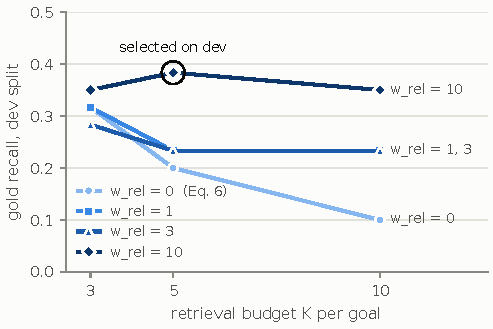
\includegraphics[width=0.86\columnwidth]{tune_relevance}
\caption{Gold recall on the development split against the retrieval budget $K$ and the weight
$w_{\mathrm{rel}}$ of the relevance term; $w_{\mathrm{rel}}=0$ is Eq.~(6).}
\label{fig:eval-tune}
\end{figure}

% Plan: the Eq. (6) finding; verdict for H3 with its power caveat.
Under Eq.~(6) as stated, development recall falls as the retrieval budget grows (0.317, 0.200 and 0.100 for
$K=3$, 5 and 10; Fig.~\ref{fig:eval-tune}): with more type-compatible candidates, the minimum-cost cover
selects the one with the fewest effects and strongest evidence however poorly it matches the goal. With
$w_{\mathrm{rel}}=10$ recall stays between 0.350 and 0.383, and on the test split removing the term lowers
recall from 0.186 to 0.082. The objective therefore needs a relevance component beside effect breadth,
evidence and declared QoS. H3 is supported for toolkit size and context cost. For gold-tool recall, a proxy
for task success, no loss is significant, but the point estimates favour every retrieval baseline and a loss
of up to 0.144 against per-subtask retrieval is not excluded.

\subsection{Certified Toolkits under Prompt Injection (H4)}
\label{sec:eval-h4}

\begin{figure*}[t]
\centering
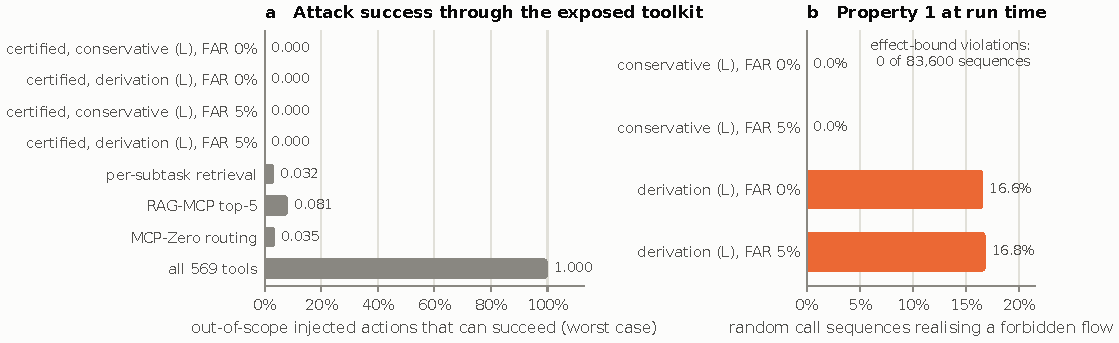
\includegraphics[width=\textwidth]{h4_injection}
\caption{(a) Worst-case success of injected actions outside the task's needed effect classes through the
exposed toolkit; 712 task--attack instances per system, with identical outcomes over three verifier seeds.
(b) Share of random call sequences over certified toolkits that realise a forbidden information flow, by how
(L) is checked.}
\label{fig:eval-h4}
\end{figure*}

% Plan: protocol; results with Wilson bounds on 712 distinct instances; what is by construction; utility price.
For each task the policy allows only the effect classes the analyst's goals require, with evidence at
$\ell_{\mathrm{obs}}$. An injected instruction then requests an action in a class the task does not need:
exfiltration (a private source together with an arbitrary-destination egress tool), deletion, code execution,
payment, or any other state change. An attack succeeds in the worst case if the exposed toolkit can truly realise it under $J$. Outcomes are identical over the three
verifier seeds, so intervals use the 712 distinct instances. Certified toolkits allow none of them at FAR 0 or
5\% (Fig.~\ref{fig:eval-h4}a; Wilson upper bound 0.54\%). Per-subtask retrieval allows 3.2\% (95\% CI
2.2--4.8\%), MCP-Zero 3.5\% (2.4--5.1\%) and RAG-MCP top-5 8.1\% (6.4--10.4\%); the full catalogue allows all. With
truthful evidence the zero rate follows from Property~1 and confirms the implementation; the baselines show
what discovery without a certificate exposes. The bound costs coverage: under these least-privilege policies
the certified toolkits reach gold recall 0.188, against 0.253--0.393 for the retrieval baselines, because the
policy also excludes tools the tasks need.

% Plan: Property 1 at run time; conservative vs derivation; truthful-label assumption; scenario 3; sanitisation.
Property~1 was also checked by executing random sequences of one to six calls over certified toolkits with the
true effects of $J$: none of 83,600 performed an effect outside $A$. Flows behave differently
(Fig.~\ref{fig:eval-h4}b): if (L) propagates labels only along the derivations recorded by the composition,
16.6\% of the sequences at FAR 0 (3,559 of 21,450) carry private data into an egress tool, because every
result returns to the context and can be written into any text argument; with the conservative reading none
does. Order independence for flows therefore requires the conservative reading, which should accompany
Property~1; these flow results take the private-output labels of $J$ as truthful verifier evidence. Under it, the
revenue scenario of Fig.~3 needs the $\chi_5$ repair, which splits the task into two toolkits, reproduces the
toolkit of Fig.~3 and hands the aggregated table over at label \emph{internal}. The sanitised manifest carries no free text and so removes description-borne injection by
construction: of 60 descriptions poisoned in the style of MCPTox~\cite{wang2025mcptox}, all reach the model in
the raw tool list and none in the manifest, which also shortens definitions from 169 to 96 tokens per tool; its
effect on selection accuracy was not measured. H4 is supported for metadata attackers; call-time
controls~\cite{debenedetti2025camel,costa2025fides,shi2025progent} remain necessary for the arguments of
permitted calls.

\subsection{Composition on Controlled Registries (RQ3)}
\label{sec:eval-rq3}

\begin{table}[t]
\caption{Composition on synthetic typed registries (RQ3): 48 tasks with hidden chains of length $L\in\{2,3,4\}$.
Valid: toolkits accepted by an independent checker, with the 95\% Wilson interval (\%). By $L$: valid share
(\%) for $L=2/3/4$. Opt.: share (\%) whose cost equals the brute-force optimum.}
\label{tab:eval-composition}
\centering\footnotesize\setlength{\tabcolsep}{2.0pt}
\begin{tabular}{@{}lrlcrr@{}}
\toprule
Regime & Valid & 95\% CI & By $L$ & Opt. & ms\\
\midrule
Exact (B\&B) & 48/48 & [92.6, 100.0] & 100/100/100 & 100 & 12.1 \\
Greedy cover & 48/48 & [92.6, 100.0] & 100/100/100 & 100 & 11.5 \\
No backward closure & 3/48 & [2.1, 16.8] & 12/6/0 & 6 & 5.2 \\
Per-subtask & 32/48 & [52.5, 78.3] & 100/100/0 & 67 & -- \\
\bottomrule
\end{tabular}
\end{table}


% Plan: generator (distractor kinds as generated), result, limits of the benchmark, interpretation.
Real registries give no ground truth for optimality, so RQ3 uses generated registries. Each task hides a typed
chain of length $L\in\{2,3,4\}$, and every step has three distractors (an unobtainable input type, lexical
evidence only, a forbidden delete effect) or, in half of the tasks, five, adding a costlier twin and a
lexically closer tool of the wrong type. The three goals name one intermediate type, the final type and a
supertype of it, so the other intermediates must be found by backward closure. A separately written checker
re-implements the reachability, effect and evidence conditions, and brute force gives the optimum.
Table~\ref{tab:eval-composition} shows that both regimes return a valid, minimum-cost toolkit for all 48 tasks
(Wilson lower bound 92.6\%) in about 12\,ms; greedy also reaching the optimum shows that these registries do
not separate the regimes. Without backward closure 3 tasks are solved. Per-subtask
retrieval, one tool per goal, solves all 32 tasks with $L\le3$ but none with $L=4$, whose chain needs more
tools than there are goals: closure over unnamed intermediate types is what completes multi-step toolkits.

\subsection{Ablations}
\label{sec:eval-ablation}

\begin{table}[t]
\caption{Request-path ablations on the LiveMCPBench test split (95 tasks). Each row changes one component of the
reference configuration; differences to the reference in parentheses. Abst.: share of tasks with an explicit
abstention.}
\label{tab:eval-ablation}
\centering\footnotesize\setlength{\tabcolsep}{3pt}
\begin{tabular}{@{}lllr@{}}
\toprule
Variant & Recall & $|K|$ & Abst.\\
\midrule
Reference (dev-tuned) & .186 & 1.42 & 0.06 \\
\midrule
No relevance term (Eq.~(6)) & .082 ($-$0.104) & 1.37 ($-$0.05) & 0.06 \\
No structural score & .173 ($-$0.013) & 1.39 ($-$0.03) & 0.07 \\
No backward closure ($d=0$) & .182 ($-$0.004) & 1.37 ($-$0.05) & 0.07 \\
No refinement (Alg.~3A) & .182 ($-$0.004) & 1.39 ($-$0.03) & 0.08 \\
Alg.~1 read literally & .175 ($-$0.011) & 1.93 (+0.51) & 0.09 \\
Strict rule~2 & .182 ($-$0.004) & 1.92 (+0.49) & 0.07 \\
Rule~1 off & .193 (+0.007) & 1.45 (+0.03) & 0.05 \\
Haiku $\rho_{\mathrm{LLM}}$ profile & .186 (+0.000) & 1.42 (+0.00) & 0.06 \\
Haiku analyst & .176 ($-$0.010) & 1.60 (+0.18) & 0.04 \\
\bottomrule
\end{tabular}
\end{table}


% Plan: interpret ablations; role ablations actually run; retrieval components.
In Table~\ref{tab:eval-ablation}, which changes one component at a time, the relevance term has by far the
largest effect. Reading Algorithm~1 literally, with only native outputs entering the context (line~15), demotes native
goals downstream of data goals and adds 0.51 tools per task, and strict rule~2 adds 0.49; both cost context
rather than coverage. Of the role ablations in the evaluation plan only the analyst's model was varied: Haiku
instead of Sonnet lowers recall by 0.010 and adds 0.18 tools. Refinement ran with its deterministic operators
only, without the assistant role; disabling it raises abstention from 6\% to 8\%. Backward closure matters
little on LiveMCPBench (recall $-0.004$), unlike on the chains of Section~\ref{sec:eval-rq3}. On all 1,509
MCPToolBench++ requests, retrieval alone reaches R@5 of 0.613 with BM25, 0.543 with the dense stand-in and
0.588 with their fusion.

\subsection{Scalability and Evolution (RQ4)}
\label{sec:eval-rq4}

% Plan: latency, Prop 3, Lemma 1, maintenance, rug pull; what of RQ4 is not covered.
Bitmap eligibility over three properties takes 1.9, 2.4 and 5.4\,$\mu$s for $10^3$, $10^4$ and $10^5$ tools,
against 1.5, 19.0 and 174.8\,ms for a scan, with identical results. Over 600 random insertions, deletions and
re-hashes against 16 cached sets, an entry was invalidated exactly when its set changed (3,615 invalidations,
5,985 entries kept, no stale answer), as Proposition~3 states for eligible sets, and
Lemma~1 held in all 300 random visibility trials. On the 569-tool registry an incremental
\texttt{list\_changed} update takes 29.9\,ms against 3.64\,s for a rebuild. A definition changed after
verification loses its observed evidence (strength 0.73 to 0.25) and regains it only when the verified
definition returns. These single runs cover the evolution part of RQ4; refinement appears only in the
ablation, and toolkit staleness was not tested.

\subsection{Contract Typing and Analyst Vocabulary}
\label{sec:eval-e8}

% Plan: what an execution-benchmark interface leaves to tau and to the analyst; single-run caveat.
Execution benchmarks such as MCP-Bench~\cite{wang2025mcpbench} pass the discovery layer only each tool's name,
description and input schema. The 525 LiveMCPTool tools were given in that form with the 95 test tasks; a task is
skipped when the selection is an abstention or empty. With lexical typing and the default policy
(read, egress and session effects), 92--99\% of the tasks are skipped whatever the analyst. With LLM-assisted
typing and an open policy, the main analyst skips 9\% (recall 0.181); a prompt whose type examples lie outside
$\Theta$ yielded out-of-vocabulary types in all 95 specifications and skips 86\%, 51\% once its vocabulary is
aligned with $\Theta$, and 36\% when it also receives the registry's domains (Algorithm~1, line~2). These single runs vary several prompt elements at once, but suggest that typing and a shared
vocabulary decide whether discovery works through such an interface. Lexical effects also over-block: on the 57 tasks whose gold tools are all read-only under $J$, the default policy skips
35\%, mostly with $\chi_2$ counterexamples (13 of 20), against 11\% under the open policy.

\subsection{Threats to Validity}
\label{sec:eval-threats}

% Plan: construct, internal, external validity, including the disclosed limitations.
\emph{Construct validity.} Exposure and attack success are measured against an LLM-labelled $J$, with no
human-labelled subset, and a simulated, non-adaptive setting: they establish soundness relative to $J$ and to
truthful verifier evidence, not that real servers behave as labelled. Gold-tool recall is a proxy for task
success that penalises inclusion-minimal toolkits when a gold chain lists alternative tools for one goal; no
task was executed end to end. \emph{Internal validity.} One model family supplied $J$, $\tau$, the analyst and
the profile, so their errors may correlate. Parameters were tuned on the development split only; the trust
policy and cost weights were fixed in advance, and $\beta$--$\zeta$, $u_{\min}$ and $d$ were not varied.
Analyst outputs are single samples, and the baselines share the weak dense encoder. \emph{External
validity.} The registries hold 569 tools, scalability uses generated contracts, and timings come from one
machine (two virtual CPUs, 7\,GB).
